\section{Основная часть}

\subsection{Подготовка виртуальной среды}

Практическая часть работы выполнялась на локальной машине с использованием Oracle VM VirtualBox. В качестве модели вычислительного кластера была использована схема из пяти виртуальных машин: один управляющий узел и четыре вычислительных узла. Управляющий узел получил имя \texttt{mgmt}, вычислительные узлы получили имена \texttt{cn01}, \texttt{cn02}, \texttt{cn03} и \texttt{cn04}.

На все виртуальные машины был установлен дистрибутив openSUSE Leap. При установке была выбрана минимальная консольная конфигурация без графической среды~--- графический интерфейс не нужен для работы служб SLURM, MUNGE и SSH, но занимает дисковое пространство и оперативную память.

Каждой виртуальной машине был выделен один виртуальный процессор и 2 ГБ оперативной памяти. Первоначально для системного диска рассматривался объём 8--10 ГБ, однако установщик openSUSE Leap для требовал не менее 12,5 ГиБ под корневой раздел и дополнительно 1--2 ГиБ под раздел подкачки. После этого виртуальные машины были пересозданы с диском объёмом 16 ГБ.

Итеративная настройка виртуальных машин оказалась важной частью работы. На раннем этапе были проверены варианты установки через openSUSE Leap Installer и выбор минимального набора пакетов. После установки управляющего узла была включена служба SSH, затем аналогичные действия были повторены на вычислительных узлах. Такой порядок позволил сначала отладить действия на одном узле, а затем перенести их на остальные машины.

\subsection{Настройка сети и доступа}

Для каждой виртуальной машины использовались два сетевых адаптера. Первый адаптер был оставлен в режиме NAT. Он нужен для доступа к внешним репозиториям openSUSE и установки пакетов через \texttt{zypper}. Второй адаптер был подключён к внутренней сети VirtualBox. Именно через этот адаптер организована локальная связь узлов кластера между собой.

Для внутренней сети был выбран диапазон \texttt{10.1.0.0/24}. Управляющему узлу назначен адрес \texttt{10.1.0.21}, вычислительным узлам назначены адреса \texttt{10.1.0.31}, \texttt{10.1.0.32}, \texttt{10.1.0.33} и \texttt{10.1.0.34}. Таким образом, осталося запас адресов для возможного расширения кластера. Также можно отметить, что назначенные адреса легко читаемые: адреса управляющих и вычислительных узлов находятся в разных десятках.

Разрешение имён выполнено через файл \texttt{/etc/hosts}. На всех узлах были добавлены одинаковые записи для имён \texttt{mgmt}, \texttt{cn01}, \texttt{cn02}, \texttt{cn03} и \texttt{cn04}. Недостатком такого подхода является необходимость синхронизировать файл на всех узлах, однако при пяти машинах это ограничение несущественно.

Следующим этапом была настройка SSH-доступа без ввода пароля. Для этого на каждом узле была создана SSH-пара ключей, публичные ключи всех узлов были добавлены в файл \texttt{/etc/authorized/keys} на каждом узле. Дополнительно был создан пользовательский SSH-конфиг, в котором имена узлов сопоставлены с соответствующими хостами и выбранным приватным ключом. После настройки команда вида \texttt{ssh cn01} выполняется с любого узла без указания ключа и без ввода пароля.

Проверка сетевого уровня выполнялась поэтапно: сначала проверялся доступ с хостовой машины к виртуальным машинам через проброшенные NAT-порты, затем проверялась связность между узлами по внутренней сети. После добавления второго адаптера необходимость открывать отдельные внешние порты для взаимодействия самих узлов отпала: SLURM и SSH внутри кластера используют внутреннюю сеть.

\subsection{Установка MUNGE и SLURM}

Для работы SLURM требуется единый механизм аутентификации сообщений между узлами. Эту функцию выполняет MUNGE. На управляющем узле был создан общий ключ MUNGE, после чего он был скопирован на все вычислительные узлы. Для ключа были выставлены ограниченные права доступа и владелец \texttt{munge}. Это важно, так как разные ключи MUNGE на узлах привели бы к отказу в обмене служебными сообщениями SLURM.

Пакеты устанавливались через пакетный менеджер \texttt{zypper}. На управляющем узле используется служба \texttt{slurmctld}, которая хранит состояние очереди, принимает задания и назначает ресурсы. На вычислительных узлах используется служба \texttt{slurmd}, которая сообщает управляющему узлу о состоянии узла и выполняет назначенные задания.

Конфигурация SLURM была сформирована через официальный конфигуратор SchedMD. В конфигурации указан кластер \texttt{practice}, управляющий узел \texttt{mgmt}, вычислительные узлы \texttt{cn[01-04]} и очередь \texttt{debug}. Для выбора процесса отслеживания был оставлен вариант \texttt{proctrack/cgroup}; для выбора ресурсов использован \texttt{select/cons\_tres}; для планировщика выбран \texttt{sched/backfill}. Эти параметры соответствуют рекомендациям конфигуратора и позволяют SLURM учитывать выделенные ресурсы, отслеживать процессы заданий и заполнять свободные промежутки в расписании.

Один и тот же файл \texttt{slurm.conf} был размещён на всех узлах в каталоге \texttt{/etc/slurm}. На управляющем узле был создан каталог сохранения состояния контроллера, на вычислительных узлах был создан каталог для состояния \texttt{slurmd}. После запуска служб проверка выполнялась командами \texttt{sinfo} и \texttt{squeue}. Узлы должны находиться в состоянии \texttt{idle}; состояние \texttt{idle*} указывает на то, что SLURM ещё не получил от узла полноценное подтверждение состояния.

\subsection{Обработка исходного набора данных}

Индивидуальный вариант определяет три параметра: дистрибутив openSUSE Leap, UID 50728 и имя задания \texttt{qe7}. Исходный набор данных был распакован и отфильтрован по UID и имени задания. В результате сформирован файл \texttt{acct\_0921-0923\_uid50728\_qe7}, содержащий 1563 записи.

В выбранном фрагменте 1542 записи имеют состояние \texttt{COMPLETED}, 11 записей имеют состояние \texttt{FAILED}, 10 записей имеют состояние \texttt{CANCELLED}. Для построения распределений использовались завершённые задания, так как только для них фактическое время выполнения можно интерпретировать как корректную длительность работы задачи.

Фактическое время выполнения задания берётся из поля \texttt{ElapsedRaw}. Ошибка прогноза времени вычисляется как разность между запрошенным временем и фактическим временем:

\[
    \Delta T = \text{TimelimitRaw} \cdot 60 - \text{ElapsedRaw}.
\]

В выбранном наборе данных минимальное фактическое время завершённого задания составляет 699 секунд, медиана составляет 1652 секунды, среднее значение составляет 1712,39 секунды. Максимальное значение равно 16660 секунд, но оно относится к хвосту распределения и не используется как типичное значение при аппроксимации. Ошибка прогноза времени для завершённых заданий имеет медиану 19948 секунд и среднее значение 19887,61 секунды. Это означает, что пользовательские задания в данном варианте обычно запрашивали существенно больше времени, чем фактически требовалось для выполнения.

На рисунке~\ref{fig:source-summary} приведена сводная визуализация исходного набора данных. Она показывает общее число записей, распределение состояний и основные характеристики времени выполнения. Этот график используется как контрольная точка: перед генерацией необходимо убедиться, что фильтрация по варианту выполнена корректно и что анализ ведётся не по всему набору данных, а именно по индивидуальной выборке.

\begin{figure}[H]
    \centering
    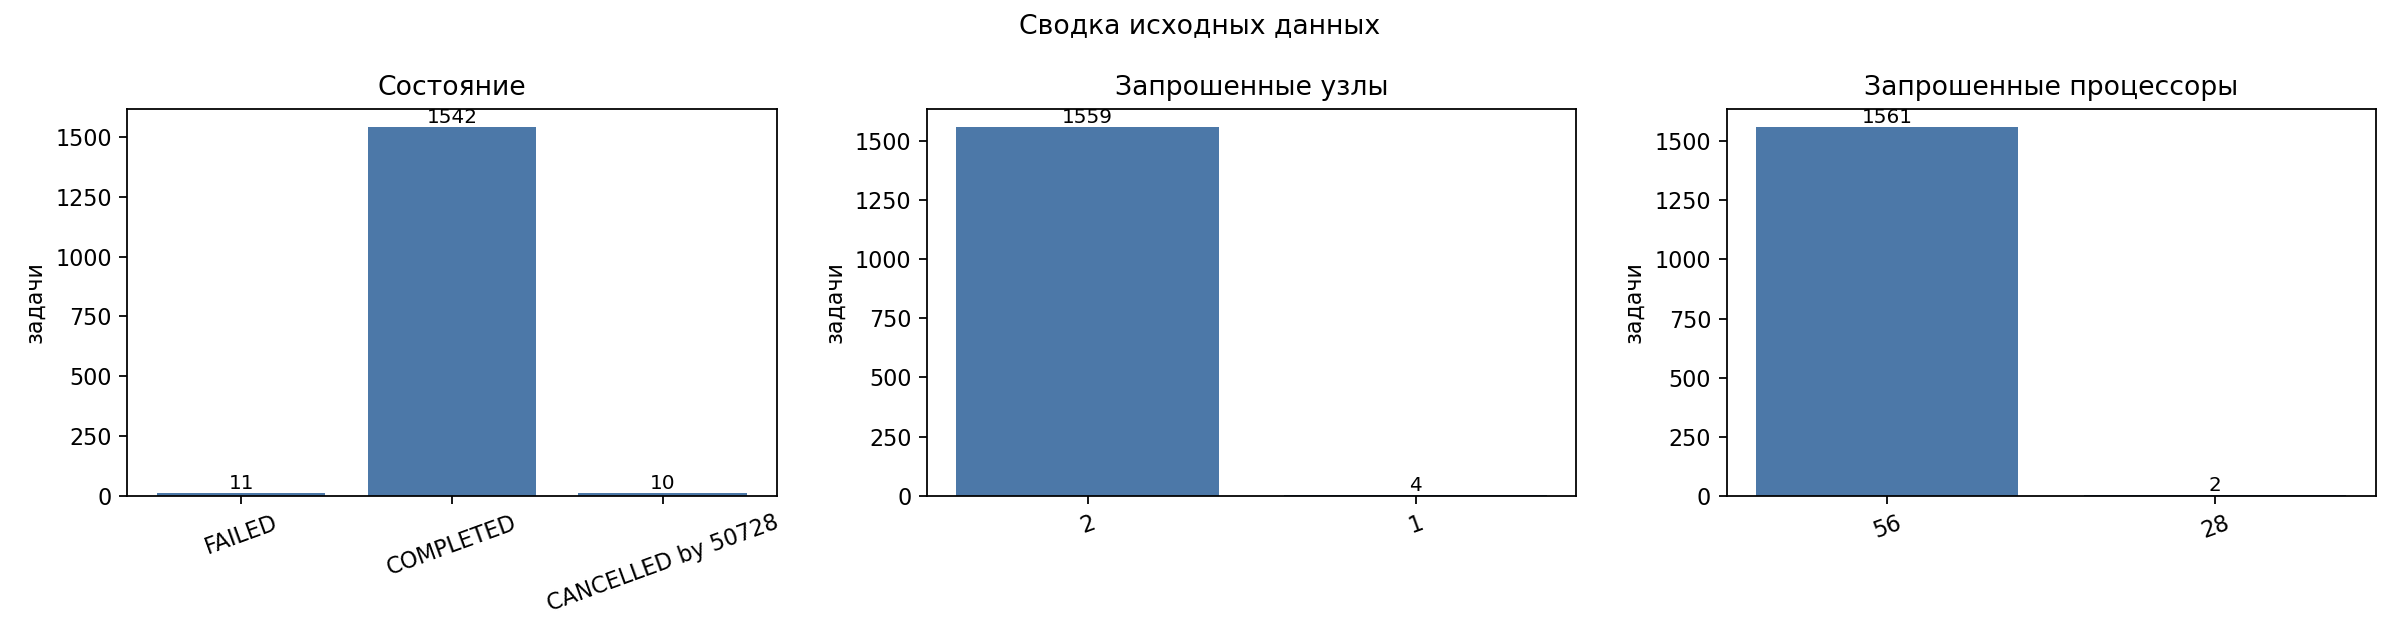
\includegraphics[width=0.92\textwidth]{../generated/graphs/source_summary.png}
    \caption{Сводка по исходному набору данных}
    \label{fig:source-summary}
\end{figure}

\subsection{Аппроксимация исходных распределений}

Анализ фактических длительностей показал, что в данных присутствуют две выраженные группы заданий. Первая группа сосредоточена около 1647 секунд и имеет вес около 0,809, вторая группа сосредоточена около 1925 секунд и имеет вес около 0,191. Поэтому фактическая длительность была описана смесью двух нормальных распределений. Параметры смеси приведены в таблице~\ref{tab:runtime-mixture}.

\begin{table}[H]
    \centering
    \caption{Параметры смеси нормальных распределений фактического времени}
    \label{tab:runtime-mixture}
    \begin{tabular}{|c|c|c|c|}
        \hline
        Компонента & Среднее, с & Стандартное отклонение, с & Вес \\
        \hline
        1 & 1647,26 & 19,89 & 0,809 \\
        2 & 1924,82 & 18,70 & 0,191 \\
        \hline
    \end{tabular}
\end{table}

На рисунке~\ref{fig:runtime-fit} показана гистограмма исходных фактических длительностей и наложенная аппроксимация смесью нормальных распределений. Видно, что одна нормальная компонента не описала бы данные корректно: между двумя группами есть заметный разрыв, а пики находятся на разных временных интервалах. Поэтому использование смеси распределений здесь оправдано содержательно, а не является усложнением ради усложнения.

\begin{figure}[H]
    \centering
    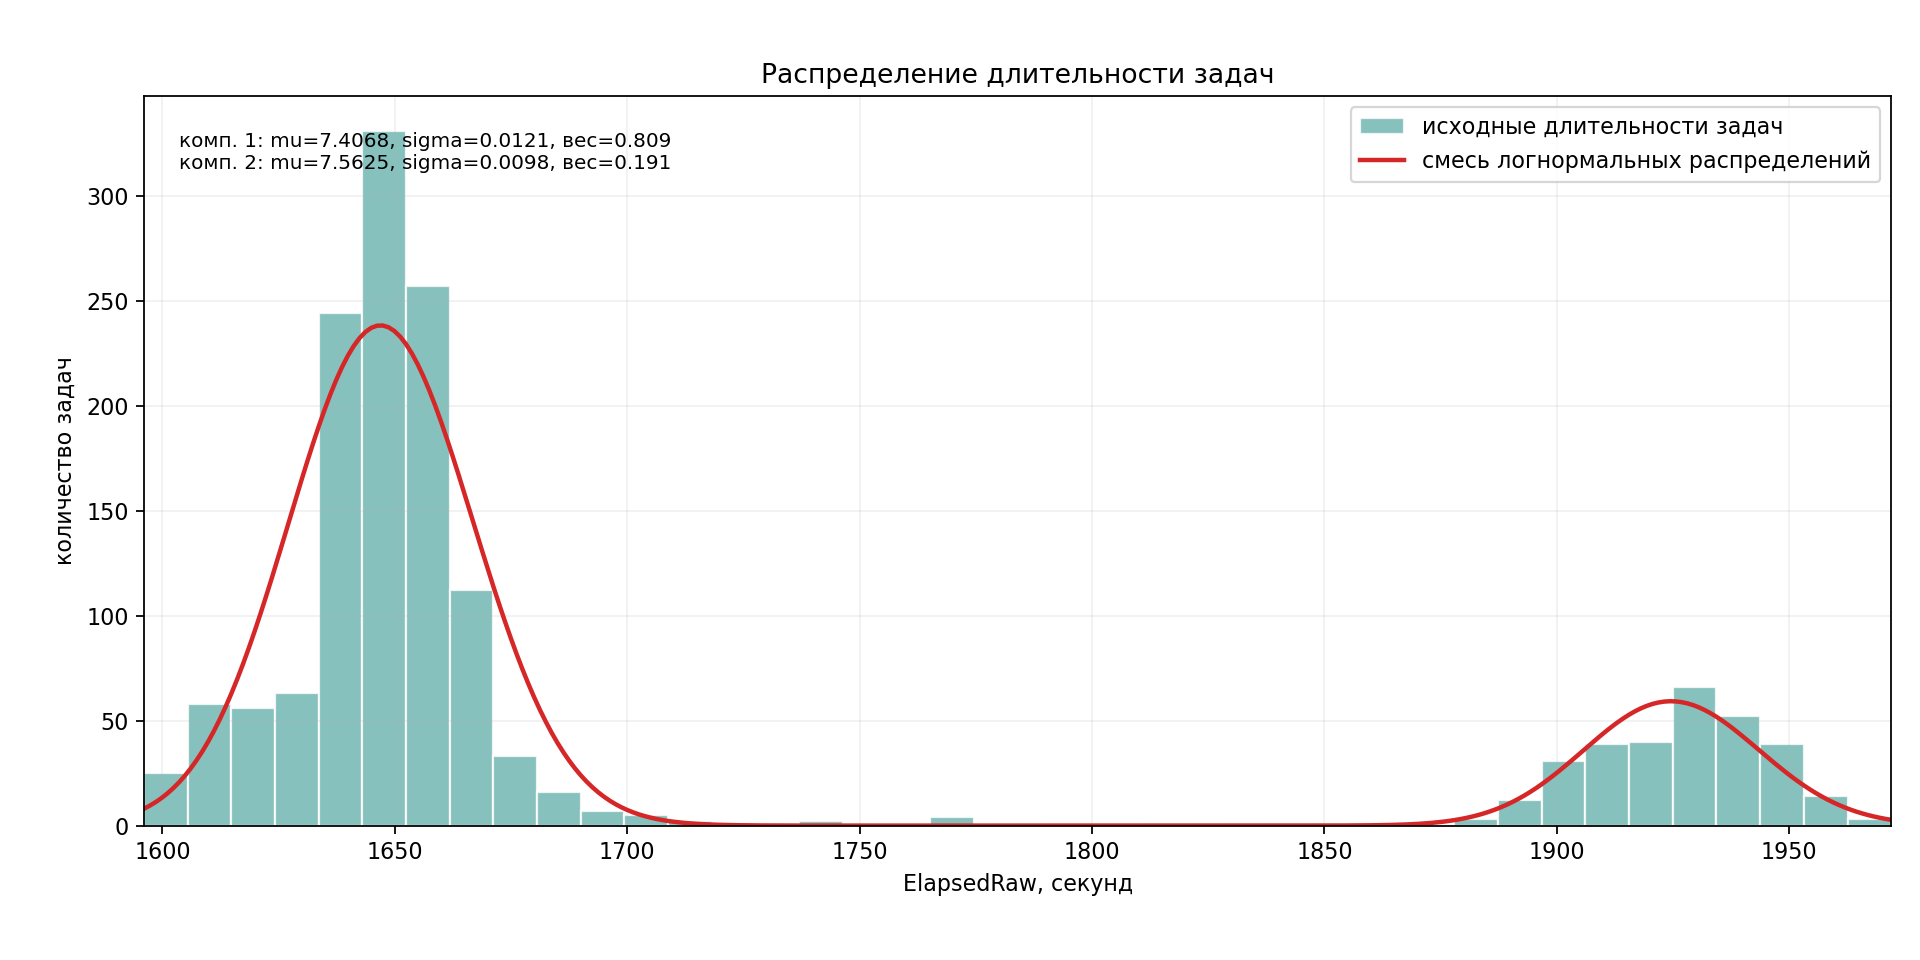
\includegraphics[width=0.92\textwidth]{../generated/graphs/runtime_fit.png}
    \caption{Аппроксимация распределения фактического времени выполнения}
    \label{fig:runtime-fit}
\end{figure}

Ошибка прогноза времени также имеет две близкие, но различимые группы. Так как ошибка является положительной величиной и рассматривается как мультипликативное отклонение, для неё используется логнормальная модель. Параметры смеси логнормальных распределений приведены в таблице~\ref{tab:error-mixture}.

\begin{table}[H]
    \centering
    \caption{Параметры смеси логнормальных распределений ошибки прогноза}
    \label{tab:error-mixture}
    \begin{tabular}{|c|c|c|c|}
        \hline
        Компонента & $\mu$ & $\sigma$ & Вес \\
        \hline
        1 & 9,8871 & 0,0014 & 0,192 \\
        2 & 9,9011 & 0,0014 & 0,808 \\
        \hline
    \end{tabular}
\end{table}

На рисунке~\ref{fig:error-fit} показано распределение ошибки прогноза времени в секундах. Столбцы гистограммы описывают исходные ошибки, красная кривая показывает логнормальную аппроксимацию. По графику видно, что ошибки сконцентрированы в районе 19,8--20,0 тыс. секунд. Это связано с тем, что в исходной выборке большинство заданий имело одинаковый или близкий лимит времени, а фактические времена выполнения отличались значительно меньше, чем сам лимит.

\begin{figure}[H]
    \centering
    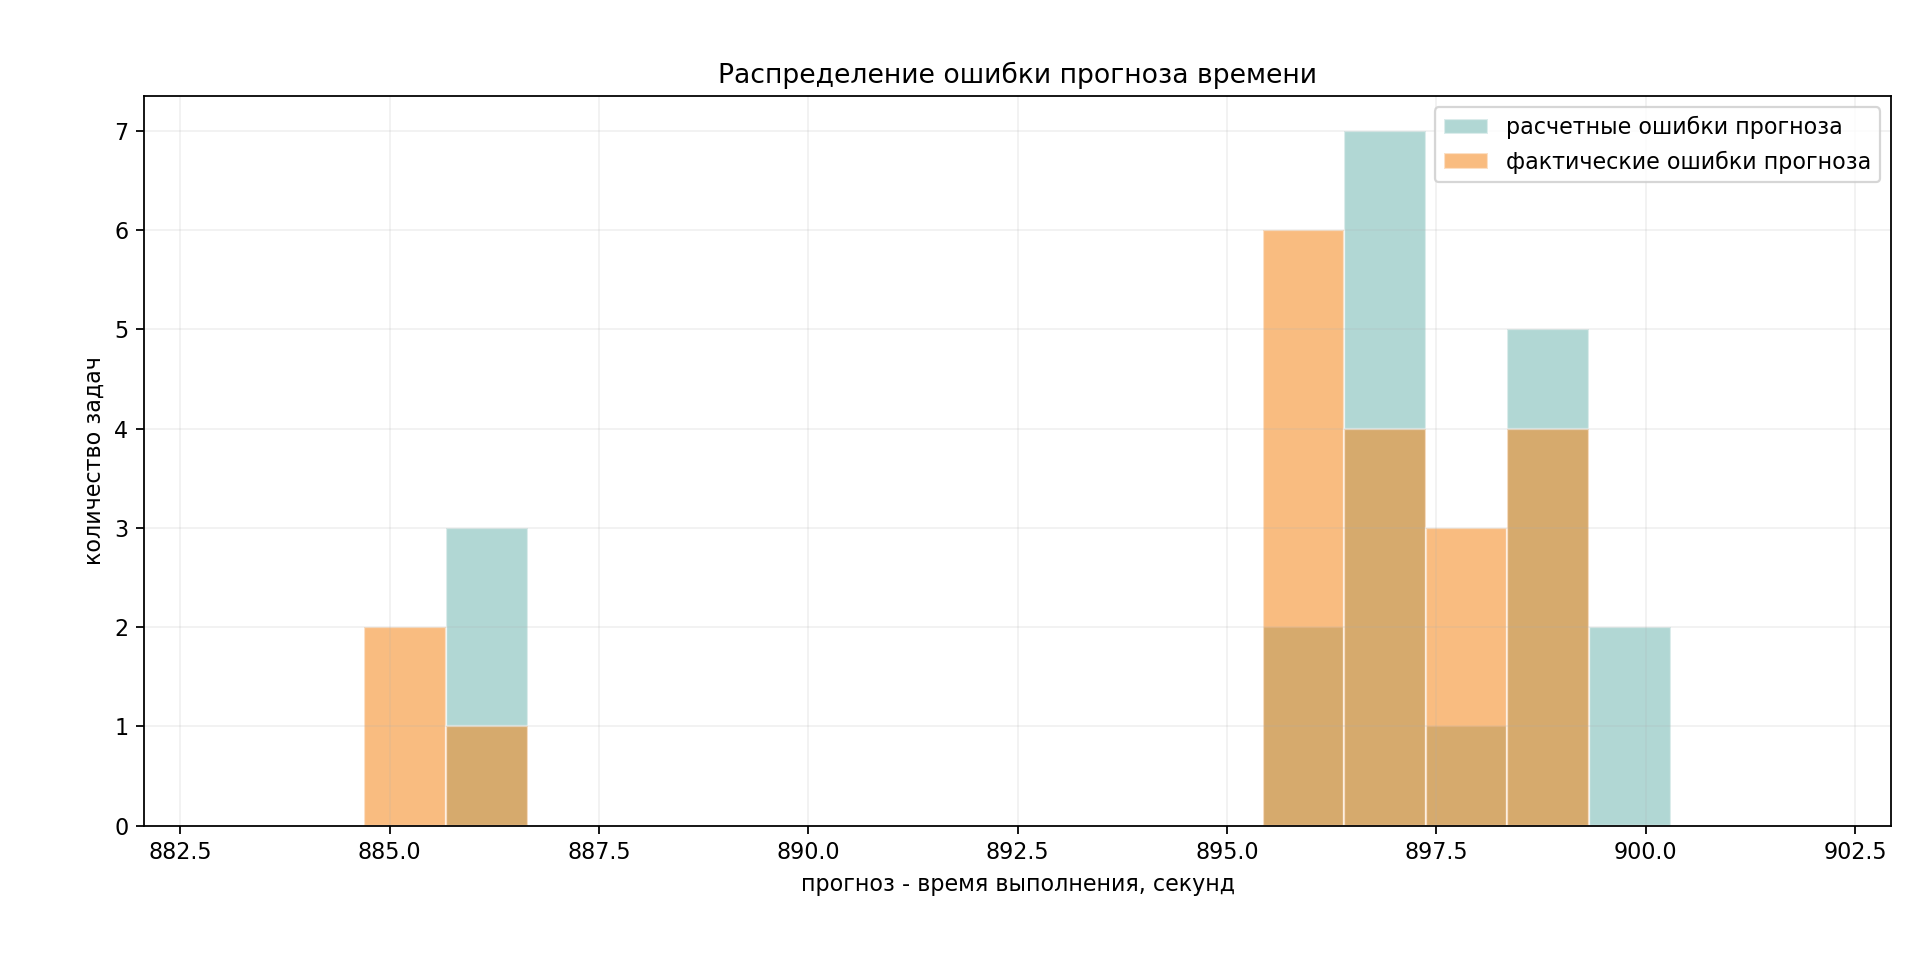
\includegraphics[width=0.92\textwidth]{../generated/graphs/forecast_error_fit.png}
    \caption{Аппроксимация распределения ошибки прогноза времени}
    \label{fig:error-fit}
\end{figure}

На рисунке~\ref{fig:log-error-fit} та же ошибка показана после логарифмирования. Такой график нужен для проверки выбранной логнормальной модели: если величина имеет логнормальное распределение, то её логарифм должен быть близок к нормальному распределению или смеси нормальных распределений. На графике видно, что две компоненты лучше различимы именно в логарифмической шкале.

\begin{figure}[H]
    \centering
    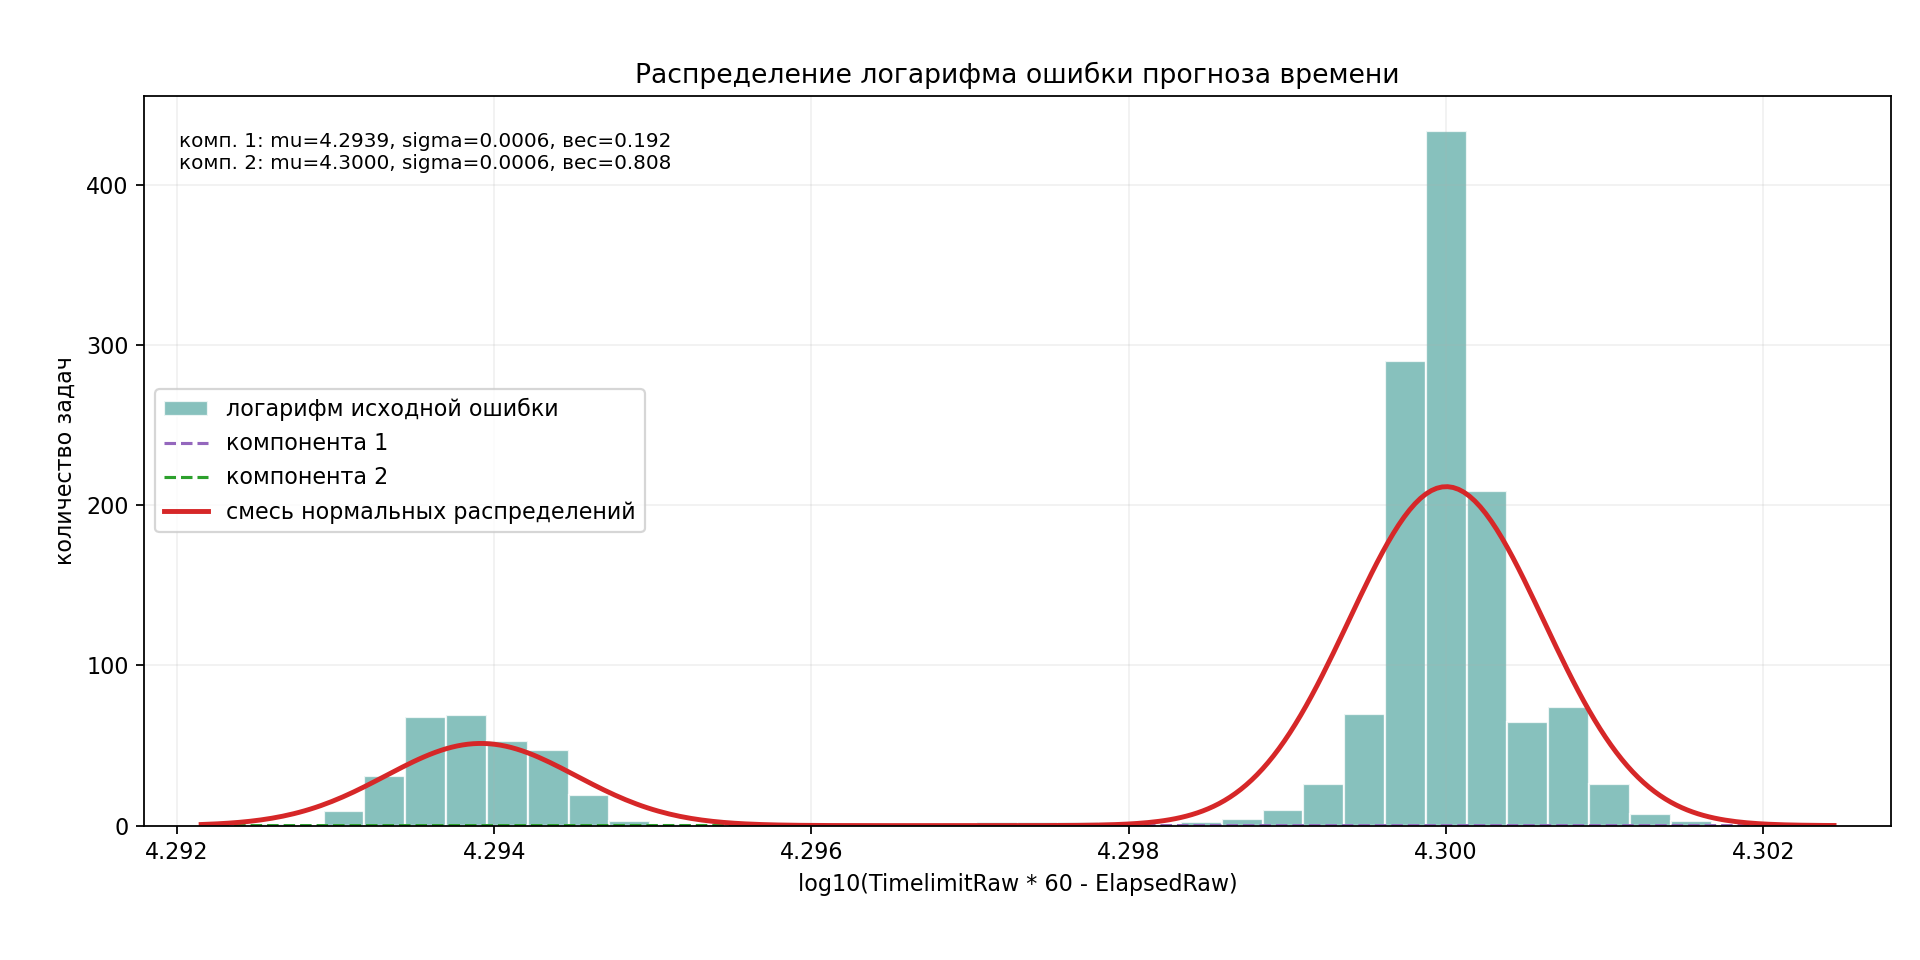
\includegraphics[width=0.92\textwidth]{../generated/graphs/log_forecast_error_fit.png}
    \caption{Распределение логарифма ошибки прогноза времени}
    \label{fig:log-error-fit}
\end{figure}

\subsection{Генерация пакетных заданий}

Генератор запускается на управляющем узле \texttt{mgmt}. На вход ему передаются число заданий, масштаб фактического времени, масштаб планового времени и параметры распределений. Для каждого задания генератор выбирает фактическую длительность по смеси нормальных распределений, выбирает ошибку прогноза по смеси логнормальных распределений, рассчитывает плановое время как сумму фактической длительности и ошибки прогноза, после чего масштабирует оба значения для практического запуска на учебном кластере.

Масштабирование необходимо, потому что исходные задания длятся десятки минут, а полный эксперимент на сотнях заданий без масштабирования занял бы слишком много времени. При этом масштабируются и фактическое время, и плановое время, поэтому относительная ошибка сохраняется. В последнем сформированном манифесте использовался масштаб около 0,045. После масштабирования медиана фактического времени \texttt{sleep} составила 74 секунды, среднее значение составило 76,116 секунды, максимум составил 89 секунд. Медиана планового времени составила 972 секунды.

Количество узлов для задания выбирается по нормальному распределению с ограничением от 1 до 4. Такой способ даёт больше заданий на 2 узла, меньше заданий на 1 и 3 узла и редкие задания на 4 узла. В манифесте на 500 заданий распределение числа узлов получилось таким, как показано в таблице~\ref{tab:nodes}.

\begin{table}[H]
    \centering
    \caption{Распределение сгенерированных заданий по числу узлов}
    \label{tab:nodes}
    \begin{tabular}{|c|c|}
        \hline
        Число узлов & Число заданий \\
        \hline
        1 & 118 \\
        2 & 245 \\
        3 & 124 \\
        4 & 13 \\
        \hline
    \end{tabular}
\end{table}

На рисунке~\ref{fig:generated-runtime} сравниваются исходное распределение фактических длительностей и сгенерированное распределение. График показывает, что генератор сохраняет две основные группы заданий. Небольшие отличия между гистограммами ожидаемы, так как генератор создаёт случайную выборку конечного размера, а не копирует исходный набор строк.

\begin{figure}[H]
    \centering
    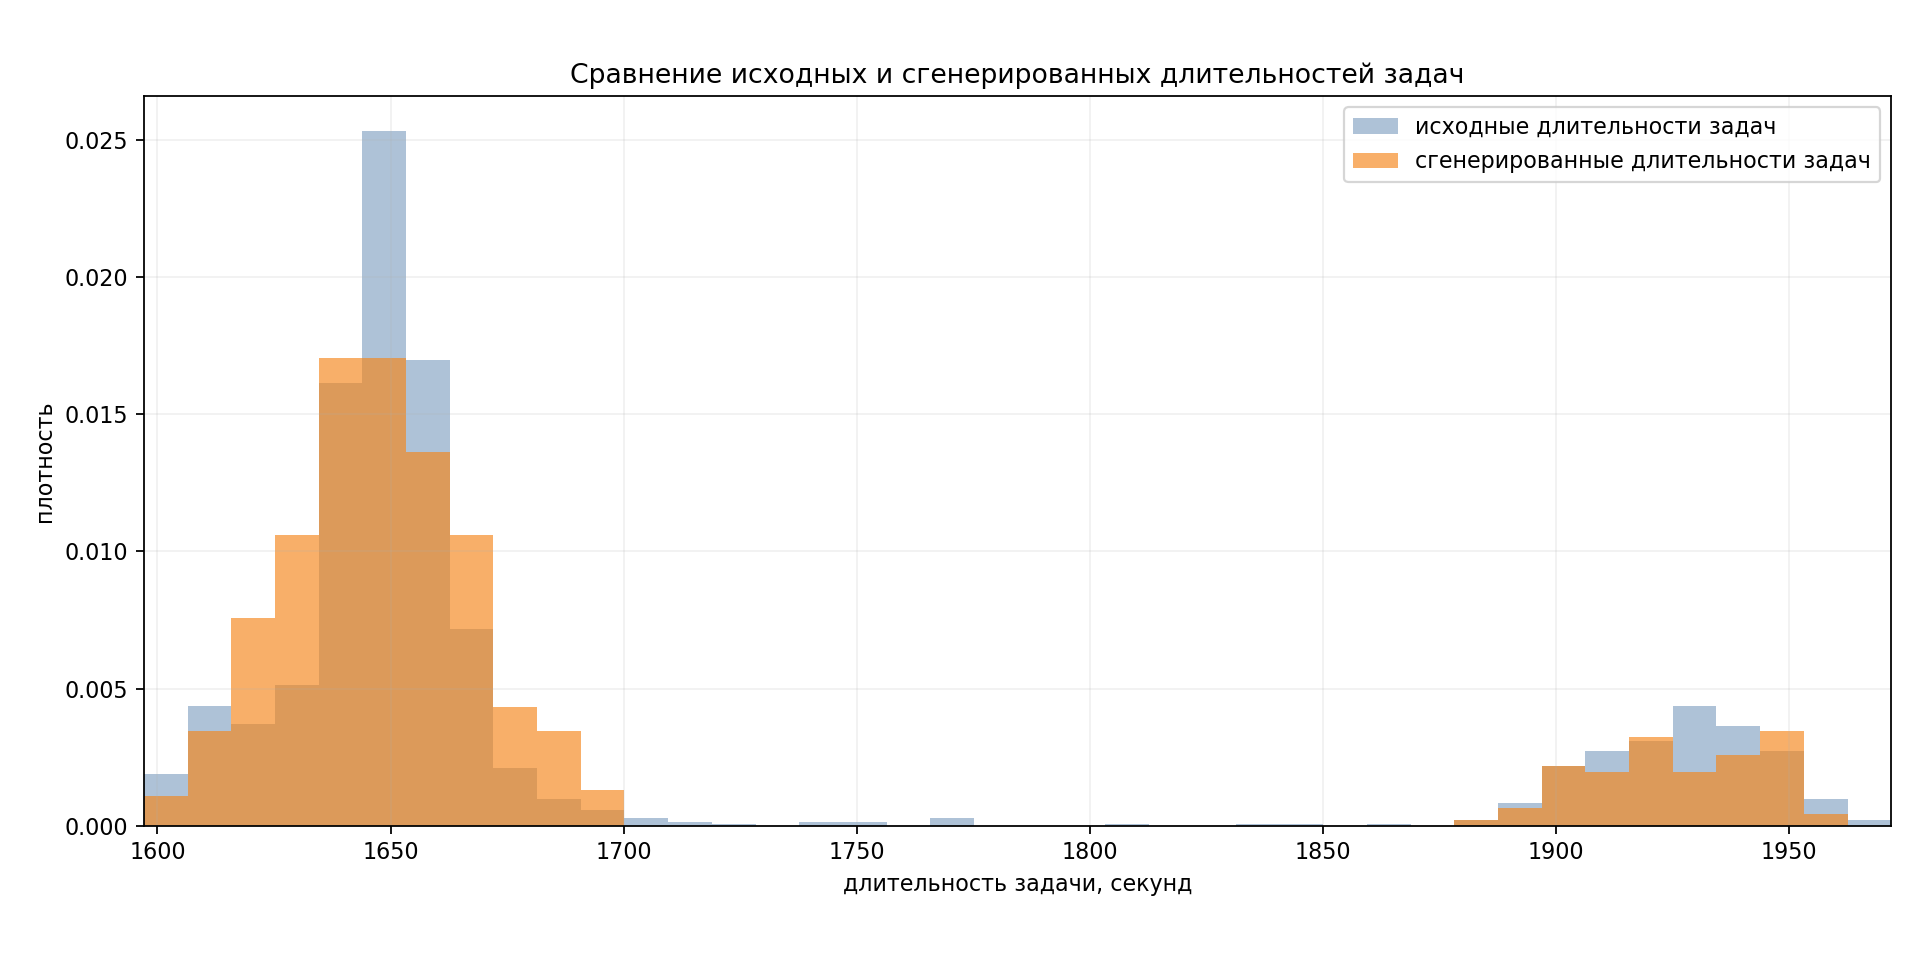
\includegraphics[width=0.92\textwidth]{../generated/graphs/generated_runtime_vs_source.png}
    \caption{Сравнение исходного и сгенерированного времени выполнения}
    \label{fig:generated-runtime}
\end{figure}

\subsection{Запуск заданий и сбор фактической статистики}

После генерации пакетные файлы отправляются в SLURM командой \texttt{sbatch}. Состояние очереди отслеживается через \texttt{squeue}, а сведения о завершённых заданиях собираются в файл \texttt{results.csv}. Для каждого задания сохраняются идентификатор SLURM, имя сценария, состояние, узел выполнения, время ожидания в очереди, фактическое время выполнения и наблюдаемое полное время.

При анализе важно разделять три величины. Первая величина~--- запланированное время из манифеста генератора. Вторая~--- значение \texttt{--time}, передаваемое в SLURM. SLURM округляет его до минут, поэтому оно не подходит для точного расчёта ошибки на коротких масштабированных заданиях. Третья величина~--- фактическое время выполнения, полученное из статистики SLURM. Поэтому для расчёта фактической ошибки используется плановое значение из \texttt{manifest.csv}, а не округлённое значение из очереди.

Полностью завершённый эксперимент на 100 заданиях показал, что все задания завершились в состоянии \texttt{COMPLETED}. Фактическое время выполнения находилось в диапазоне от 16 до 21 секунды, медиана составила 17 секунд. Накладные расходы относительно команды \texttt{sleep} в этом коротком эксперименте имели медиану около 5,57\%. Для более длинного запуска на 500 заданий уже завершённая часть показала меньшие относительные накладные расходы: медиана около 1,15\%. Это ожидаемо, потому что постоянная задержка запуска и завершения задания слабее влияет на более длинные задания.

На рисунке~\ref{fig:planned-actual} показано сравнение планового и фактического времени по отдельным заданиям. Плановое время заметно больше фактического, что соответствует исходной задаче моделирования: пользователь заранее запрашивает лимит времени с большим запасом, а реальное выполнение завершается раньше. На графике также видно, что фактическое время меняется в узком диапазоне, так как масштабированные задания выполняют только команду \texttt{sleep}.

\begin{figure}[H]
    \centering
    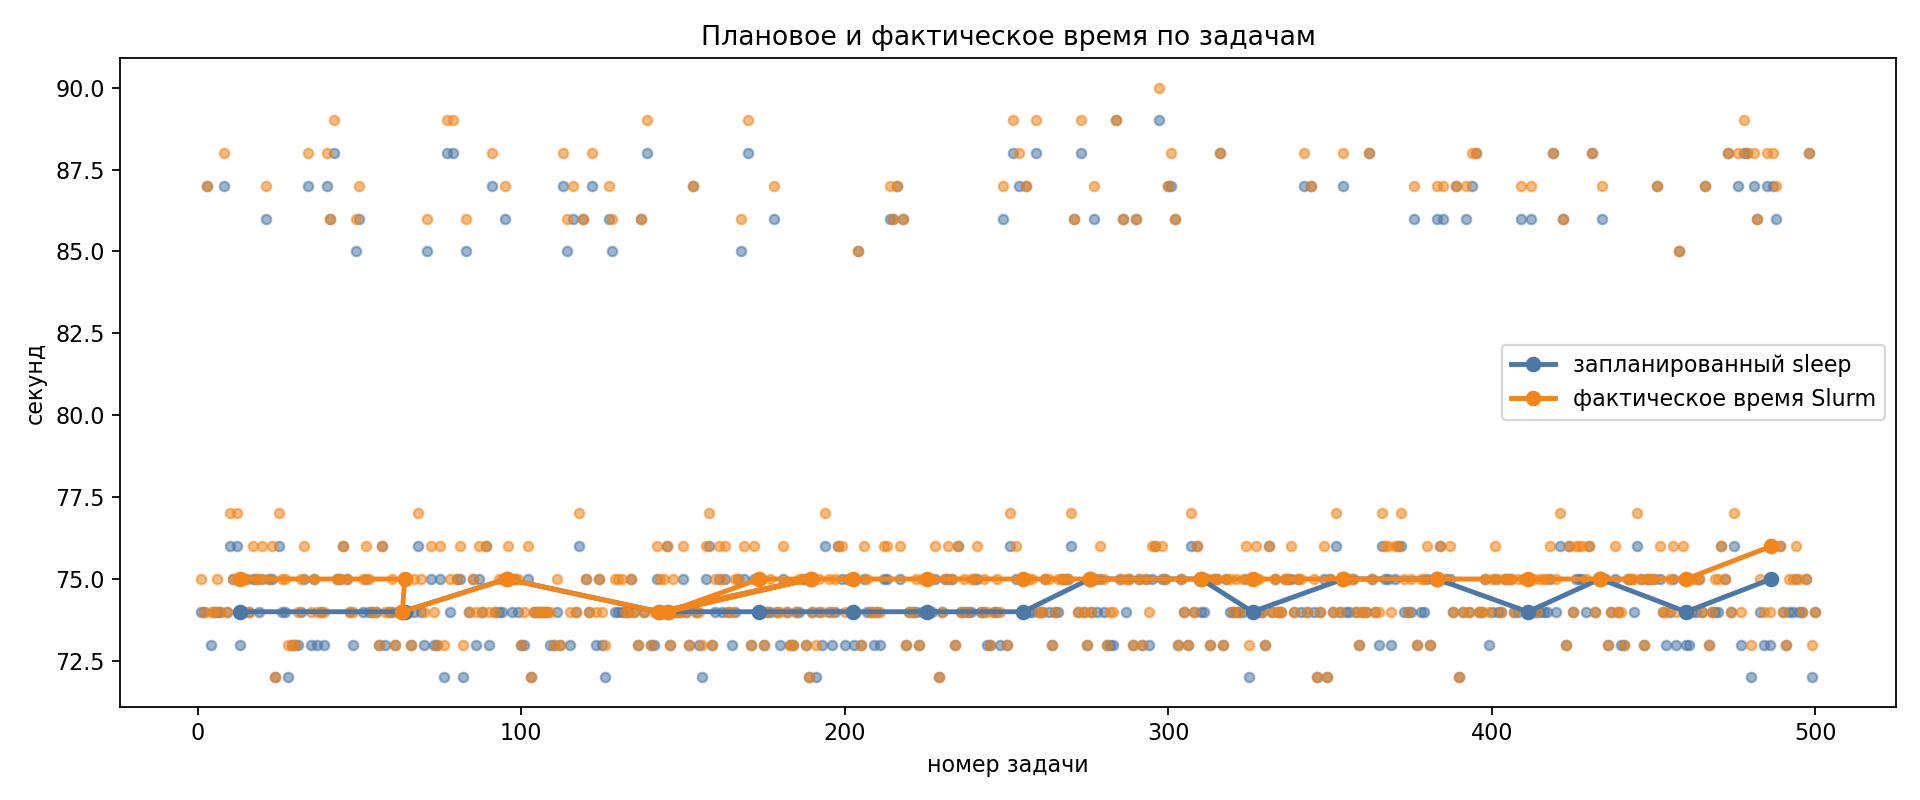
\includegraphics[width=0.92\textwidth]{../generated/graphs/planned_vs_actual_by_job.png}
    \caption{Плановое и фактическое время выполнения заданий}
    \label{fig:planned-actual}
\end{figure}

На рисунке~\ref{fig:actual-runtime-spread} показан разброс фактического времени выполнения заданий. Этот график нужен для проверки стабильности эксперимента: если бы часть заданий выполнялась существенно дольше ожидаемого, это означало бы влияние внешних факторов или перегрузку виртуальной среды. В завершённом эксперименте разброс небольшой, а значения группируются около запланированного времени \texttt{sleep} с добавлением небольшой постоянной задержки.

\begin{figure}[H]
    \centering
    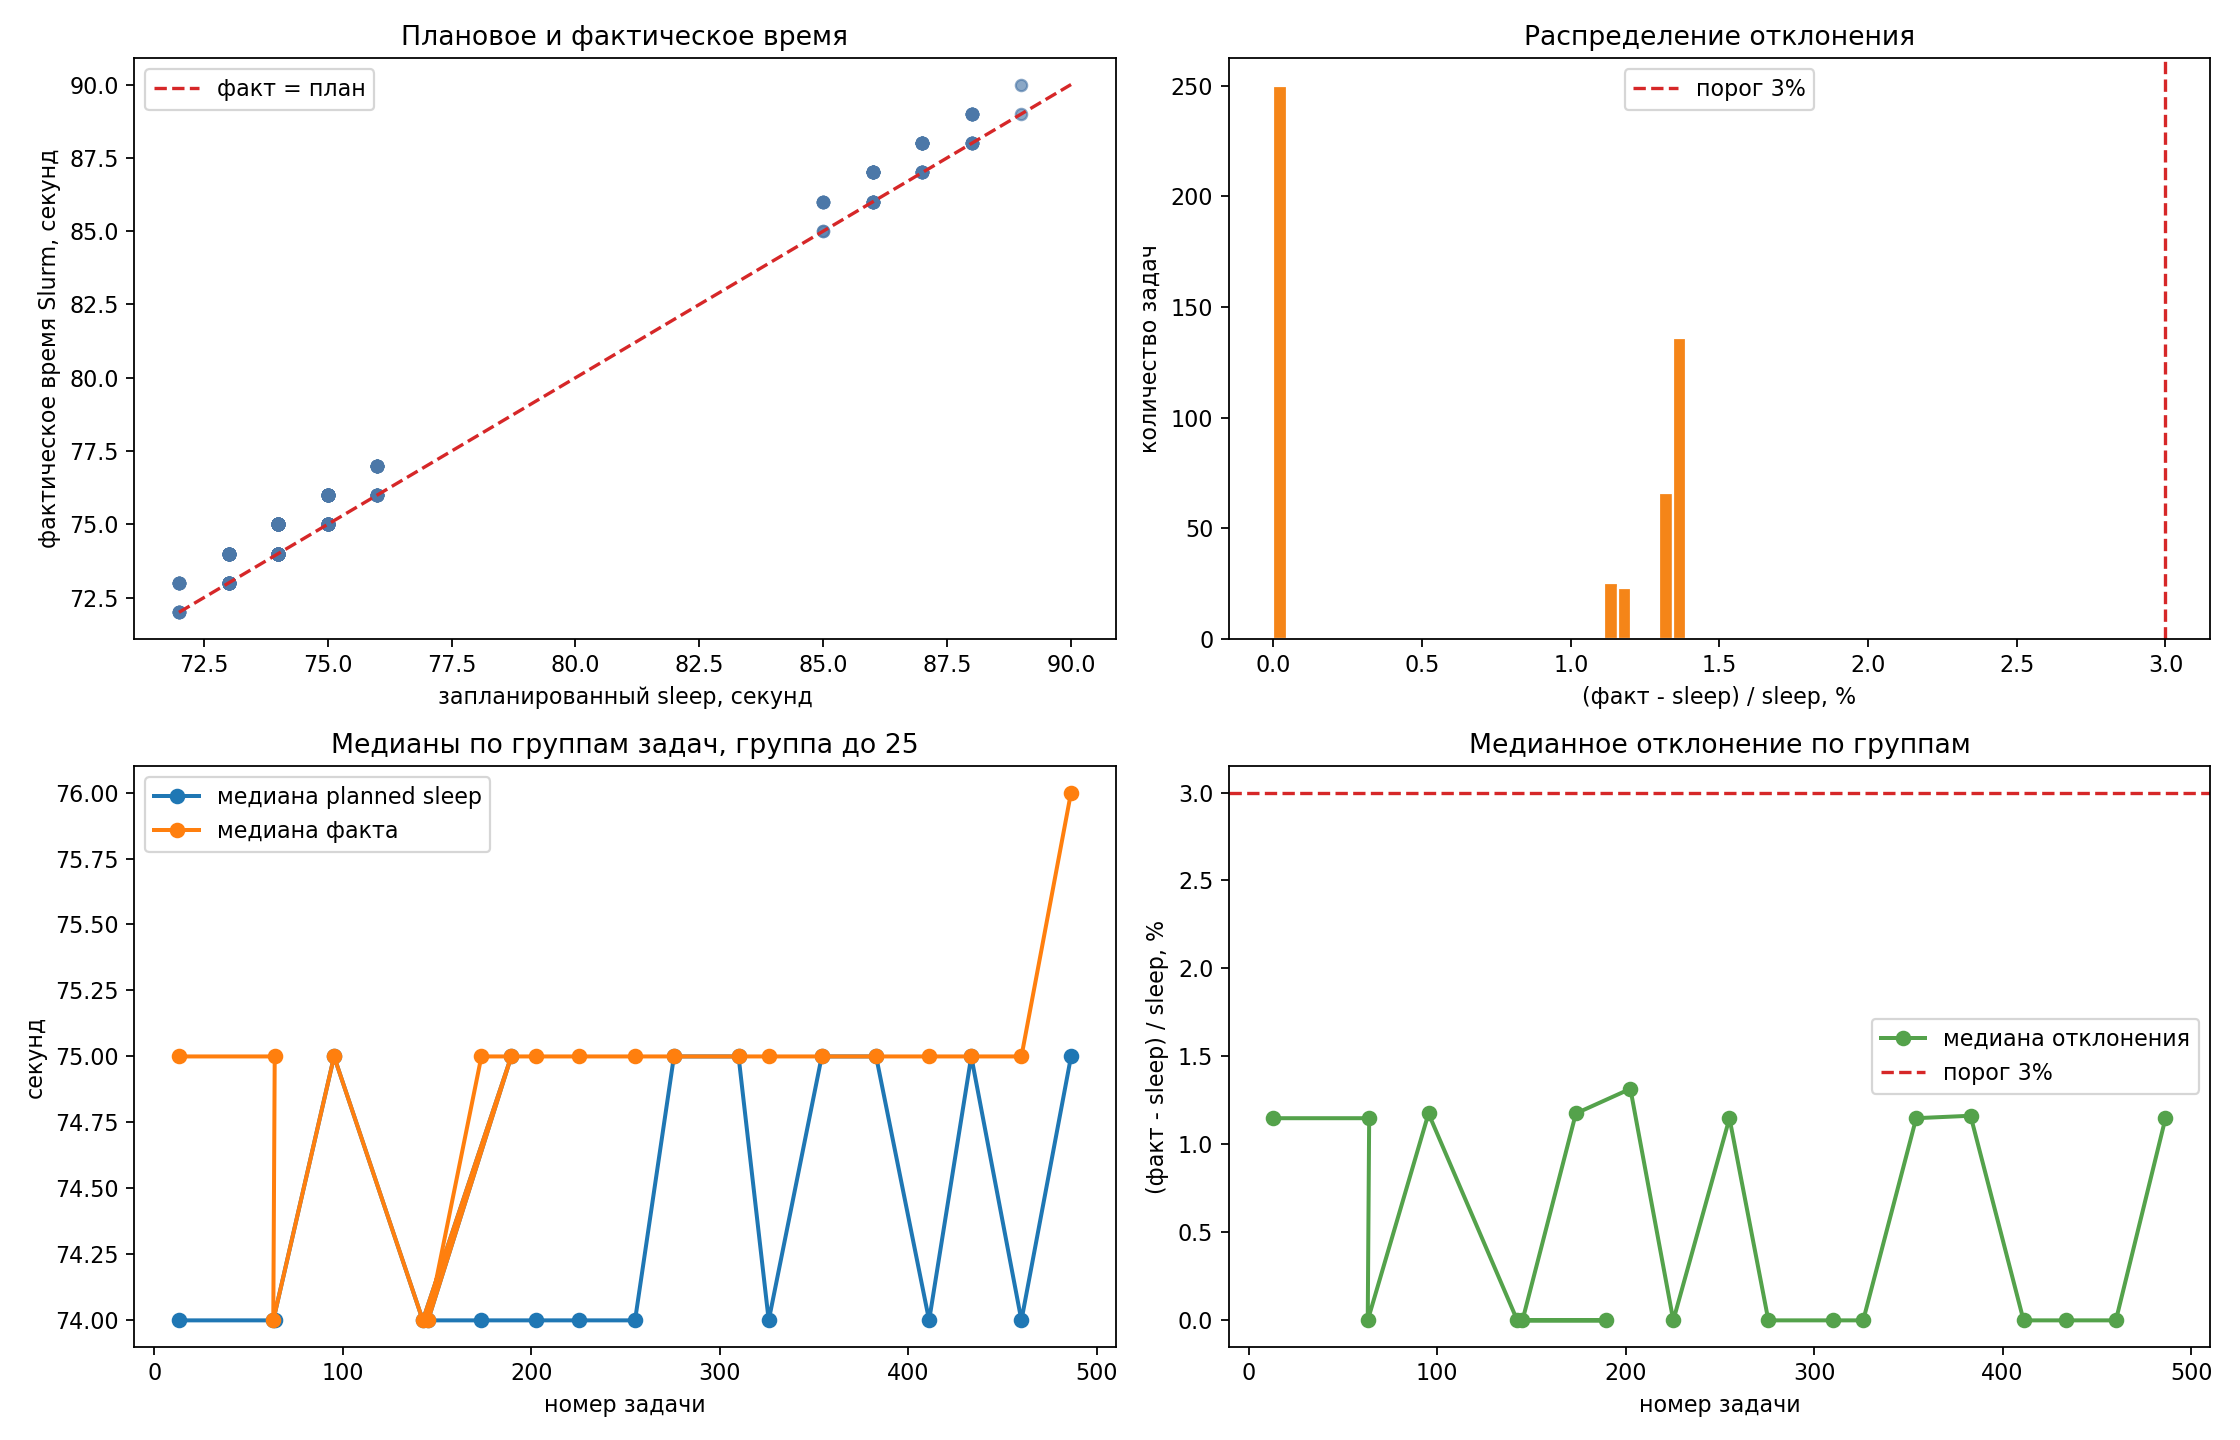
\includegraphics[width=0.92\textwidth]{../generated/graphs/actual_runtime_spread.png}
    \caption{Разброс фактического времени выполнения заданий}
    \label{fig:actual-runtime-spread}
\end{figure}

На рисунке~\ref{fig:actual-overhead} показано отклонение фактического времени от времени \texttt{sleep}. Этот график позволяет оценить накладные расходы SLURM и виртуальной среды. В коротком запуске даже 1 секунда дополнительного времени даёт заметный процент, поэтому для финального длительного запуска был увеличен масштаб времени. Это позволяет удерживать относительное отклонение около 2\% и не получать выбросы выше 3\%.

\begin{figure}[H]
    \centering
    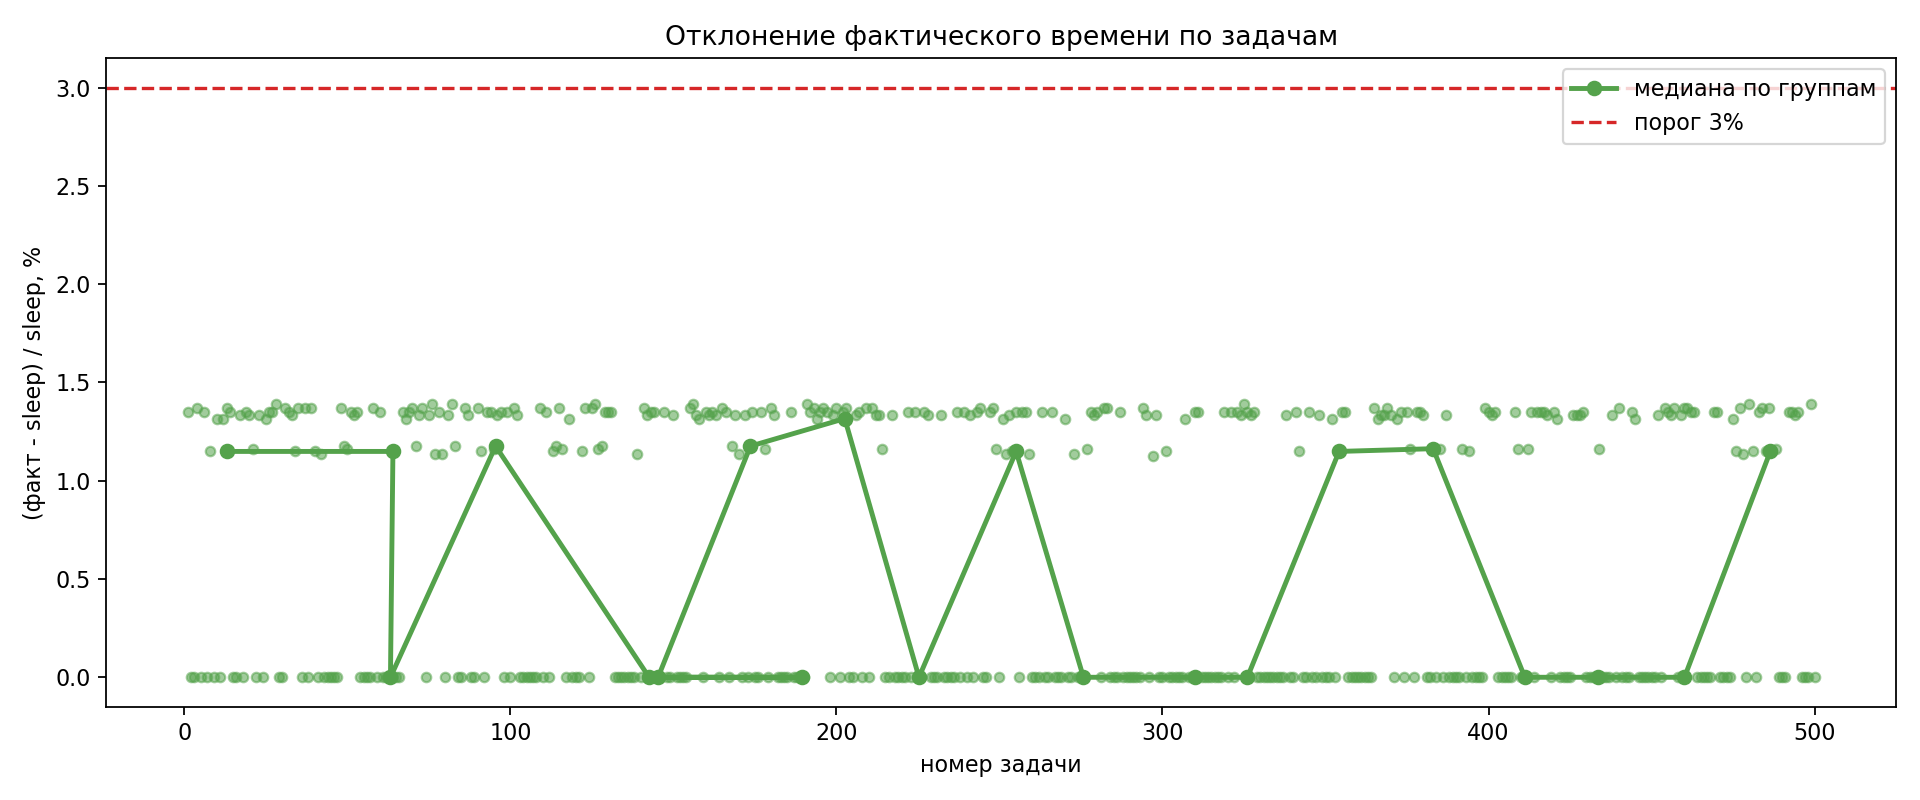
\includegraphics[width=0.92\textwidth]{../generated/graphs/actual_overhead_by_job.png}
    \caption{Накладные расходы фактического выполнения по заданиям}
    \label{fig:actual-overhead}
\end{figure}

\subsection{Анализ фактической ошибки прогноза}

После получения фактического времени выполнения можно пересчитать ошибку прогноза уже не для исходных данных, а для выполненных на кластере заданий. Эта величина определяется как разность между масштабированным плановым временем из манифеста и фактическим временем выполнения, полученным из SLURM.

На рисунке~\ref{fig:actual-error-fit} показано распределение фактической ошибки прогноза. В завершённом запуске на 100 заданий ошибка находилась примерно в диапазоне от 190 до 206 секунд, медиана составила около 196 секунд. Форма распределения остаётся компактной, потому что плановое время было сгенерировано из той же модели, а фактическое время отличается от \texttt{sleep} в основном на небольшую постоянную задержку.

\begin{figure}[H]
    \centering
    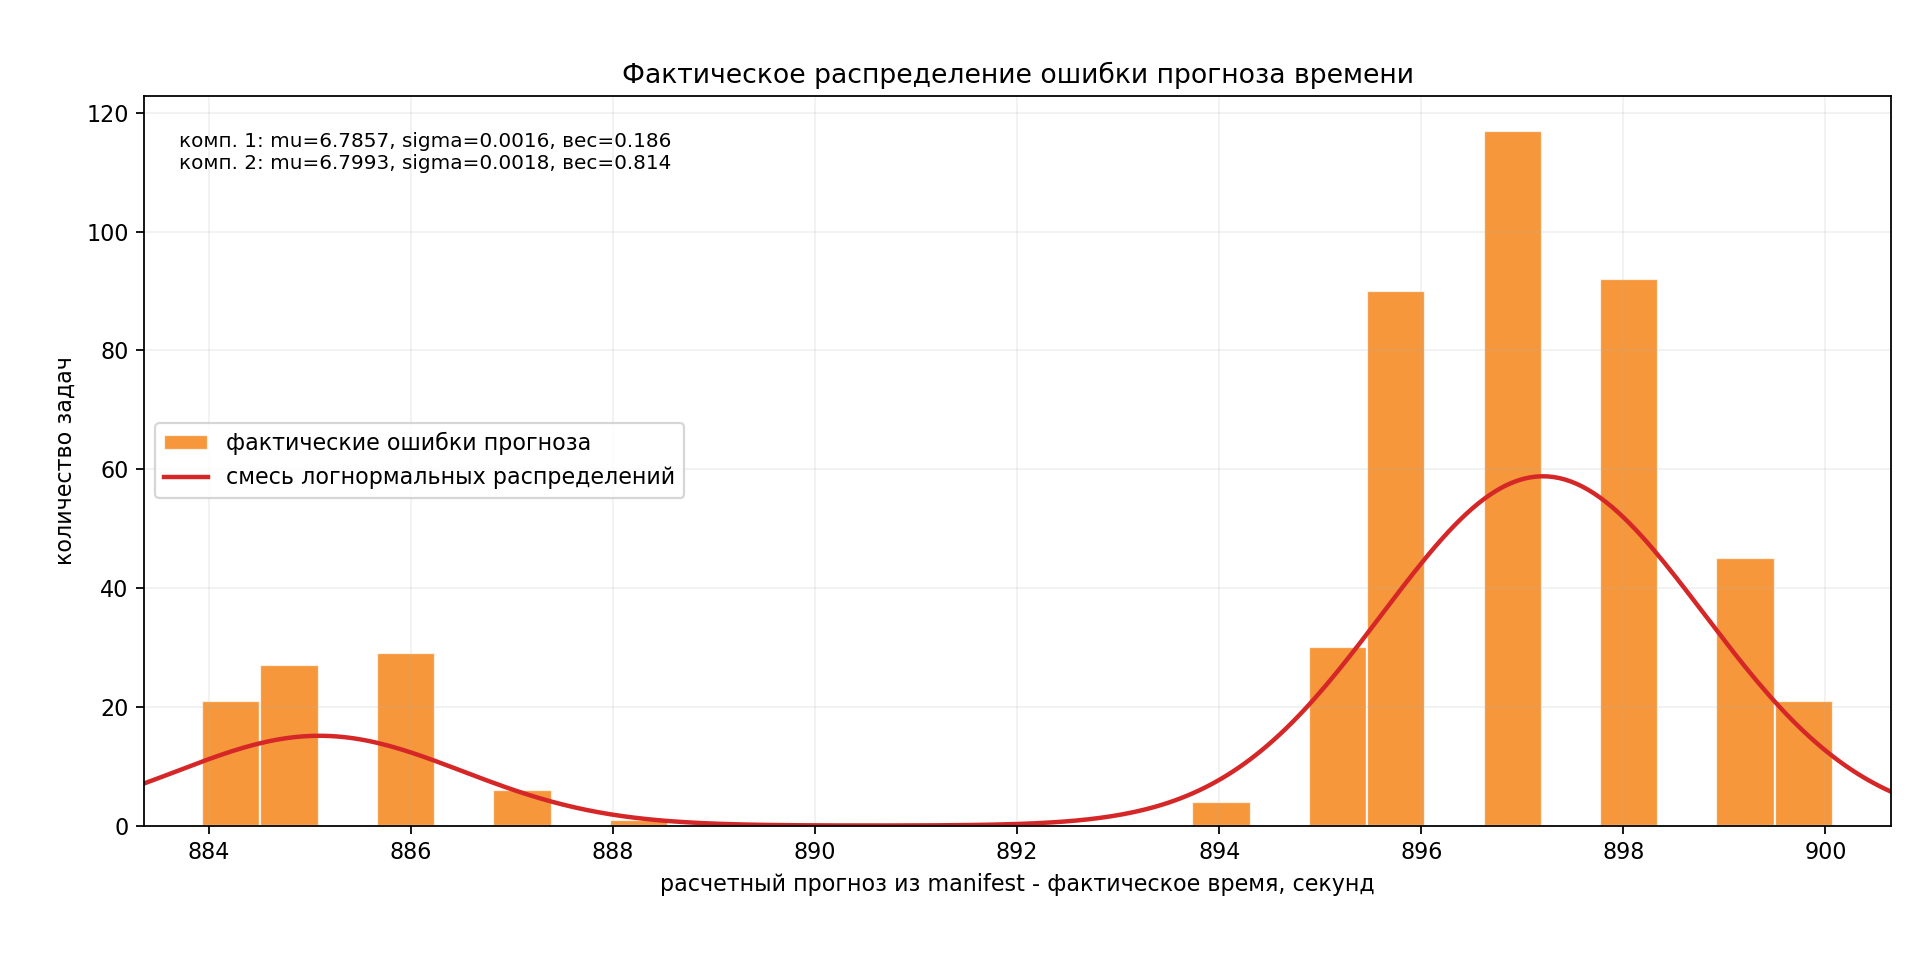
\includegraphics[width=0.92\textwidth]{../generated/graphs/actual_error_fit.png}
    \caption{Распределение фактической ошибки прогноза времени}
    \label{fig:actual-error-fit}
\end{figure}

На рисунке~\ref{fig:log-actual-error-fit} показан логарифм фактической ошибки прогноза. Как и для исходных данных, логарифмическая шкала используется для проверки логнормальной природы ошибки. Наложенная кривая показывает, что после выполнения на кластере ошибка сохраняет форму, близкую к той, которая была заложена генератором, но становится немного сдвинутой из-за накладных расходов выполнения.

\begin{figure}[H]
    \centering
    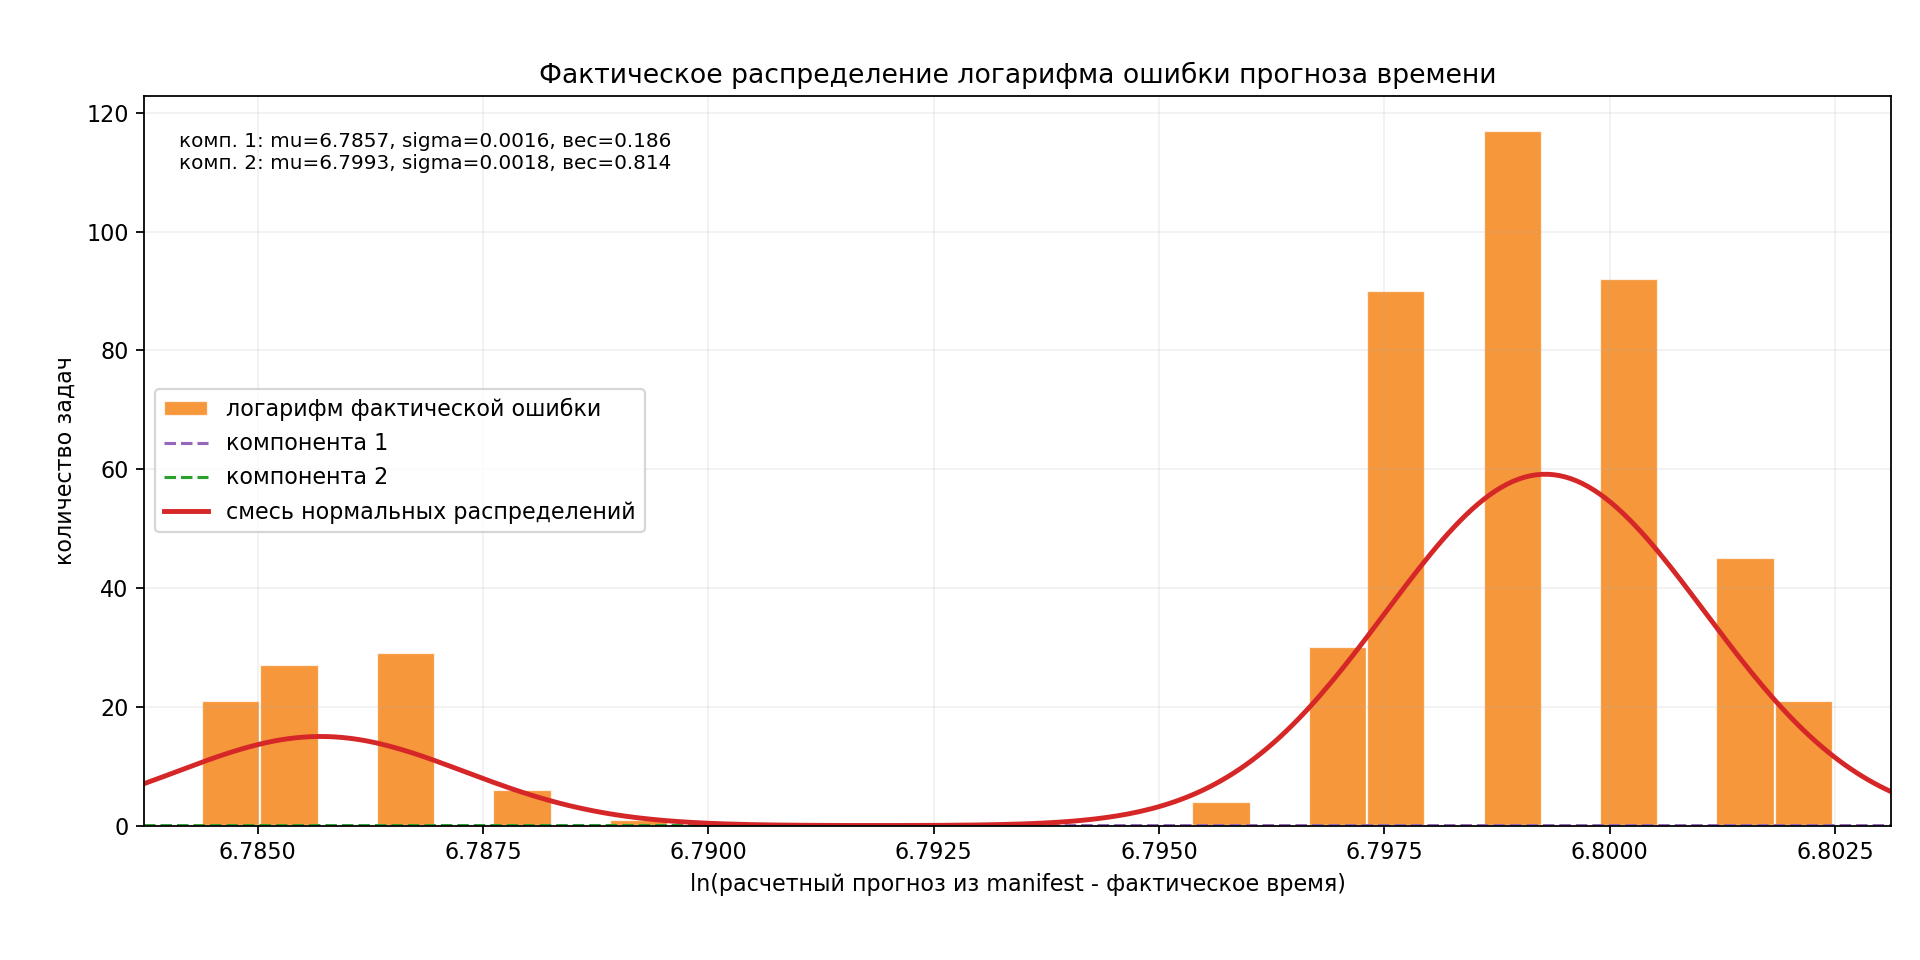
\includegraphics[width=0.92\textwidth]{../generated/graphs/log_actual_error_fit.png}
    \caption{Распределение логарифма фактической ошибки прогноза времени}
    \label{fig:log-actual-error-fit}
\end{figure}

Для манифеста на 500 заданий была выполнена оценка длительности полного запуска. При четырёх вычислительных узлах ожидаемая длительность составляет около 6,5 часов. Если считать накладные расходы равными 1,5 секунды на задание, медианное относительное отклонение фактического времени от планируемого составляет около 2,03\%, а максимальное отклонение остаётся меньше 3\%. Поэтому выбранный масштаб подходит для длительного эксперимента: запуск остаётся выполнимым за одну ночь и при этом относительное влияние накладных расходов не искажает результаты слишком сильно.
